\subsection{Expérience pratique avec calcul de force}
Une expérience pratique simple à réaliser avec ce système consiste à mesurer la force de maintien maximale. Cette force correspond à la force maximale que le piège optique peut appliquer pour maintenir une particule dans sa position. L'expérience a été effectuée avec un mélange d'eau distillée et de crème pour les mains (de la marque Nivea), comme proposé dans le manuel d'utilisation fourni par Thorlabs.

Ci-dessous, une liste énumérée expliquant chaque étape avec les calculs nécessaire pour déterminer cette force :

\vspace{1em}
\begin{minipage}{0.6\textwidth}
    \begin{enumerate}
        \item La première étape consiste à connaître le ratio pixels/\textmu m. Pour cela, on mesure une bille de silice dont son diamètre réel est connu : 2,06~\textmu m, et son diamètre dans l'image est de 34 pixels. On obtient donc le ratio suivant :
              \[
                  \text{ratio} = \frac{34~\text{pixels}}{2.06~\text{\textmu m}} = 16,50~\text{pixels/\textmu m}
              \]
        \item On sélectionne ensuite une particule de graisse quelconque et on mesure son diamètre dans l'image (Figure~\ref{mesure_bead}). Cette particule de graisse mesure 136 pixels de diamètre. En utilisant le facteur précédent :
              \[
                  R = \frac{136}{2 \cdot \text{ratio}} = 4,12~\text{\textmu m}
              \]
        \item Toujours avec la même particule, on mesure la vitesse maximale où la particule reste encore piégée par le faisceau laser. Une vitesse maximale de 0,065~mm/s a été mesurée.
    \end{enumerate}
\end{minipage}
\hfill
\begin{minipage}{0.38\textwidth}
    \centering
    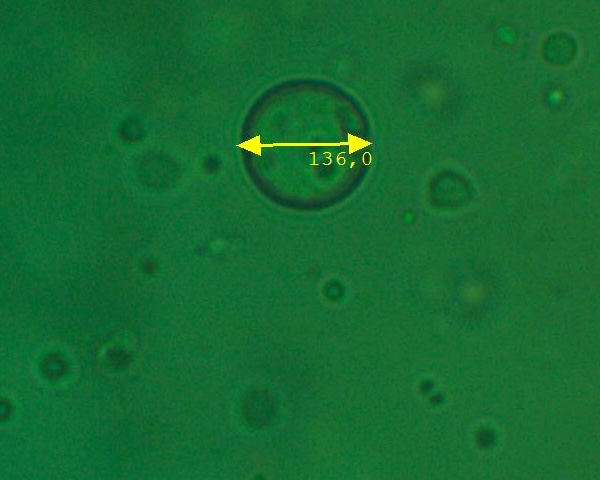
\includegraphics[width=\textwidth]{assets/figures/Notice de laboratoire/mesure_bead.jpg}
    \captionof{figure}{Mesure d'une particule du mélange eau distillée/crème en pixels}
    \label{mesure_bead}
\end{minipage}
\newpage
Une fois toutes ces mesures réalisées, la force de maintien maximale \( F_R \) peut être calculée avec l'équation suivante :
\begin{equation}
    F_R = 6 \pi \eta_{\text{eff}} R v \tag{1}
\end{equation}
\myequations{Force de maintien maximale pour une particule.}
\textbf{Légende :}
\begin{itemize}[label=\textbullet]
    \item $\eta_{\text{eff}}$ : viscosité effective du milieu liquide
    \item $R$ : rayon de la particule
    \item $v$ : vitesse linéaire de la particule dans le liquide
\end{itemize}

\textbf{Calcul numérique :}
\[
    F_R = 6 \pi \cdot 1{,}003 \cdot 10^{-3}~\text{Pa}\cdot\text{s} \cdot 4{,}12 \cdot 10^{-6}~\text{m} \cdot 6{,}5 \cdot 10^{-5}~\text{m/s} = 5{,}06~\text{pN}
\]

\section{Observations avec différents mélanges}
Un mélange d'eau distillée avec du dentifrice au charbon noir (de la marque Primark) a été testé. Sur la figure~\ref{dentifrice_charbon}, on peut apercevoir à ce qui s'apparente à un fragment de charbon noir. Un phénomène surprenant se produit au moment où le laser touche une particule noire : au lieu d'être attirée vers le centre du faisceau laser, elle est repoussée.

\begin{figure}[H]
    \begin{center}
        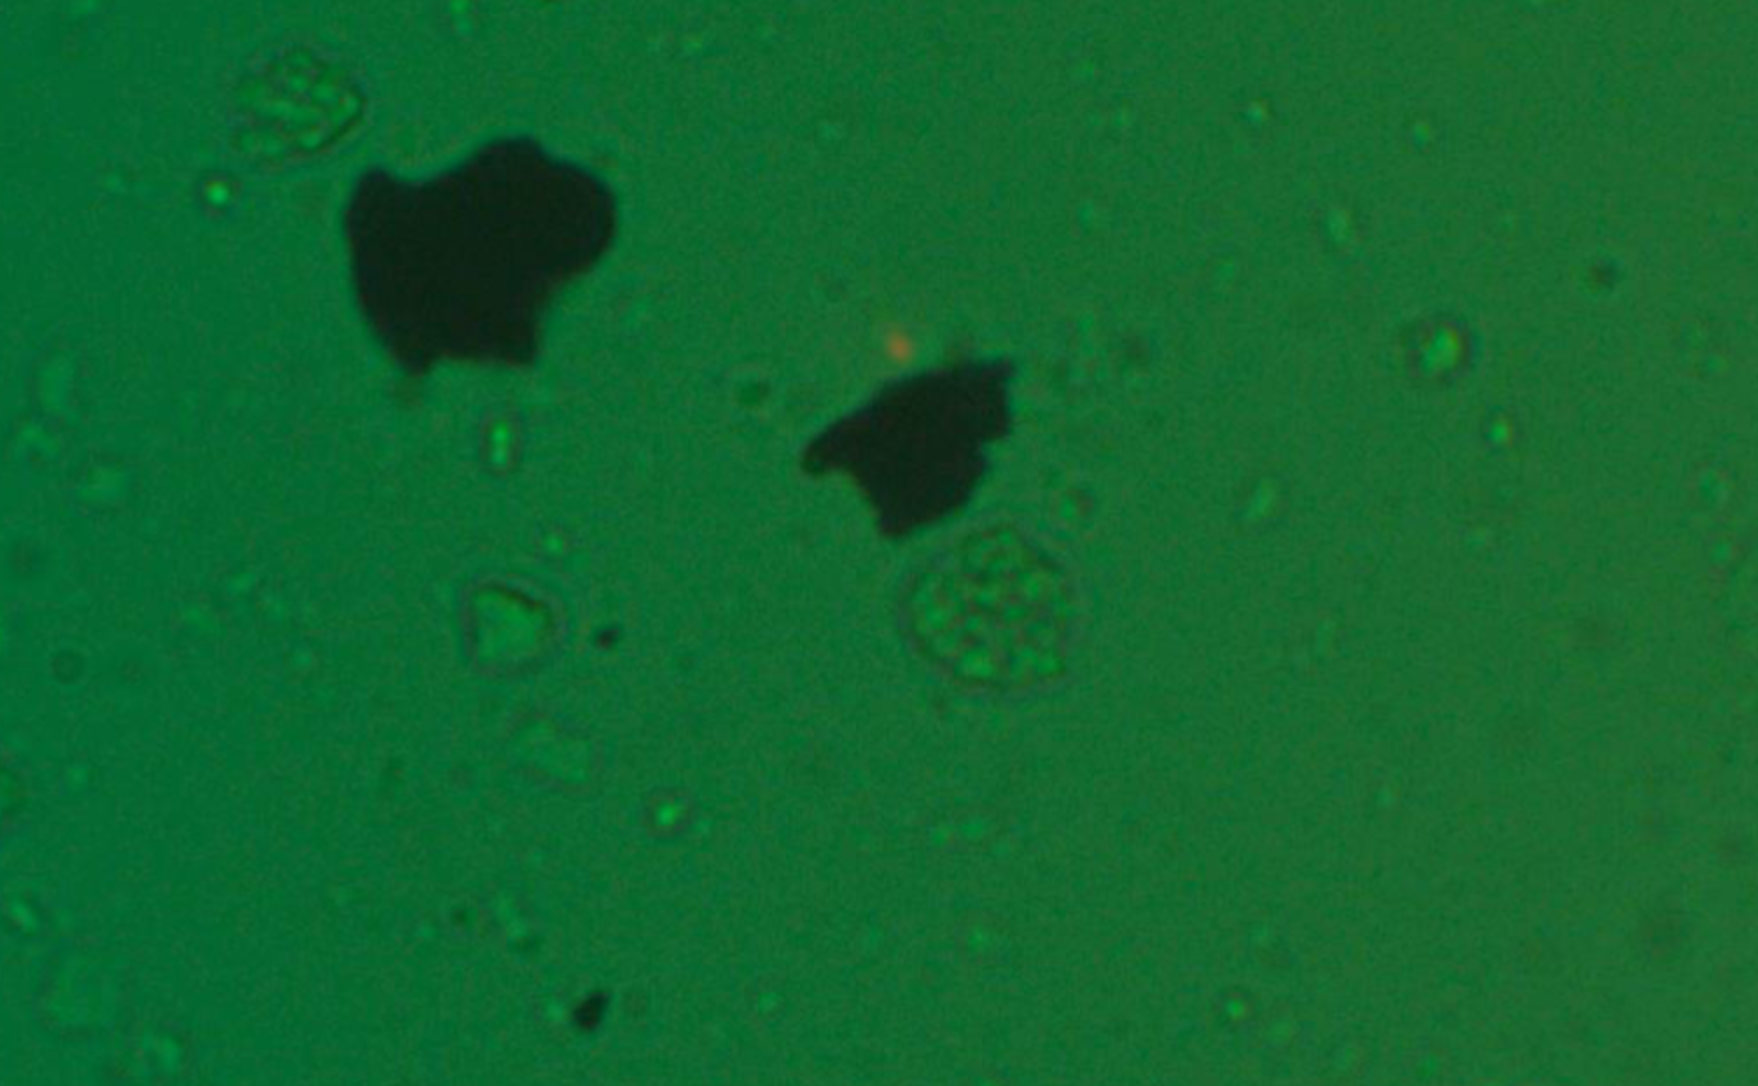
\includegraphics[width=0.7\textwidth]{assets/figures/Notice de laboratoire/dentifrice_charbon.png}
    \end{center}
    \caption{Mélange d'eau distillée avec du dentifrice au charbon noir}
    \label{dentifrice_charbon}
\end{figure}

Ce comportement peut s'expliquer par le fait que la matière noire absorbe fortement la lumière. Contrairement aux particules transparentes qui sont attirées vers le centre du faisceau à cause de la force de gradient, les particules noires, comme le charbon, sont surtout influencées par une force de diffusion. Cette force vient du fait que la particule absorbe une grande partie de la lumière et crée une poussée dans la direction du faisceau. Résultat : au lieu d'être attirée, elle est repoussée par le laser.

\newpage
\section{Contenu de la notice}
Ce système doit pouvoir être exploré par des étudiants lors d'un cours au sein du laboratoire COMATEC-LANS. Étant donné que le manuel d'utilisation du système fourni par Thorlabs comprend 108 pages au total~\cite{manualPortableOpticalTweezers}, il semble nécessaire de concevoir une notice de laboratoire plus compacte, afin de faciliter sa prise en main. La notice complète se trouve en annexes à la page~\pageref{annexe:notice_labo_Kinesis_ThorCam}. Ci-dessous, une liste résumée du contenu de cette notice.

Cette notice de laboratoire est structurée de manière à guider pas à pas l'utilisateur qui souhaite découvrir ce système de pinces optiques.
% La notice est divisée en six parties principales. Elle commence par une présentation détaillée du système et de ses éléments de sécurité. Ensuite, un guide d'installation des logiciels nécessaires (ThorCam et Kinesis) est proposé. La préparation de l'échantillon est expliquée étape par étape, suivie du réglage précis de sa position verticale pour un piégeage efficace. Une partie est ensuite consacrée à la manipulation des particules, accompagnée d'un exemple de calcul de force. Enfin, la dernière section décrit les étapes pour remettre le système en ordre à la fin de l'expérience.
Elle est organisée selon les phases suivantes :

\begin{enumerate}
    \item \textbf{Présentation des composants du système} : description détaillée des éléments constituant le système, avec un intérêt particulier sur les dispositifs de sécurité pour que l'utilisateur puisse facilement les identifier et comprendre leur rôle.

    \item \textbf{Installation et prise en main des logiciels} : guide pas-à-pas pour l'installation des logiciels ThorCam et Kinesis, accompagnée d'une explication claire de leur rôle dans la capture d'image et le contrôle des moteurs.

    \item \textbf{Préparation de l'échantillon} : protocole pour préparer correctement l'échantillon, afin de garantir une manipulation optimale par la pince optique.

    \item \textbf{Réglage précis de la position verticale de l'échantillon} : méthodes pour ajuster la position verticale de la lame dans le système, afin d'optimiser le focus du laser et assurer un piégeage efficace des particules.

    \item \textbf{Expériences de positionnement de particules} : réalisation d'expériences de déplacement des particules à l'aide de la pince optique, avec un calcul détaillé permettant d'estimer la force maximale exercée par le laser pour maintenir les particules piégées.

    \item \textbf{Remise en ordre du système} : Explications pour éteindre, nettoyer et ranger le matériel en fin d'utilisation.
\end{enumerate}

Une notice pour la même expérience, mais en utilisant le logiciel ServoVision est également disponible en annexes à la page~\pageref{annexe:notice_labo_ServoVision}.